%!TEX TS-program = xelatex
%!TEX encoding = UTF-8 Unicode
%!TeX spellcheck = it_IT
%!TEX root = ../tesi.tex

\chapter{Simulazioni}\label{chap:simulazioni}
% INTRO: cosa c'è in questa sezione?
Dopo aver illustrato il protocollo in esame e il modello di propagazione utilizzato, si passa ora alla fase di valutazione.
Il capitolo procederà, quindi, nel dettaglio dei diversi scenari affrontati illustrando
le motivazioni che hanno portato alla loro realizzazione, definendone i parametri e motivando i risulati ottenuti.
%
\section{Configurazione a griglia}\label{sec:configurazione-griglia}
% \subsection{Panoramica}
% Simulazioni codice barichello:
%  - struttura simulazioni
%  - grafici
%  - risulati
Il primo gruppo di simulazioni ha lo scopo di analizzare l'impatto degli edifici sul comportamento del protocollo
Fast Broadcast all'interno di uno scenario conosciuto, ossia quello presentato nella tesi originale~\cite{Barichello2017propagazione}
a cui sono stati aggiunti degli edifici creati apposititamente.
La configurazione dello scenario, dei nodi e della rete è la stessa ed è riassunta in Tabella~\ref{tab:parametri-simulazioni-barichello}.
L'ambiente è una città fittizia con strade a griglia in stile Manhattan di lunghezza $4000$ metri e distanti l'una dall'altra $300$ metri.
I veicoli sono disposti a $12$ metri di distanza per un totale di $8064$.
Il veicolo che da inizio alla fase di inoltro (generazione del primo messaggio di inoltro),
che per facilità verrà chiamato veicolo \textit{zero}, è posizionato al centro della griglia.
Seguendo l'idea originale, è stata definita anche un circonferenza di raggio pari a $1000\pm12$ metri, utilizzata per definire alcune metriche che verranno descritte in seguito;
la circonferenza ha centro in corrispondenza del veicolo zero.
Il raggio trasmissivo effettivo (fisico) assume due valori possibili: $300$ o $500$ metri;
%
\begin{table}[!h]
	\centering
	\begin{tabular}{| L{.4\linewidth} | r  l |}
		\toprule
		Parametro															&			Valore 							&					\\
		\thickerline
		Lunghezza delle strade								&			$4000$							& m				\\
		Distanza fra le strade								&			$300$								& m				\\
		Distanza fra i veicoloi								&			$12$ 								& m				\\
		Circonferenza													&			$1000\pm12$					& m				\\
		Posizione del veicolo zero						&			centrale						&					\\
		\thickerline
		Dimensioni pacchetto									&				$164$							&			byte		\\	\hline
		Standard tramissione									&				$802.11$b					&							\\	\hline
		Frequenza															&				$2.4$							&			GHz			\\	\hline
		Banda del canale											&				$22$							&			MHz			\\	\hline
		Velocità di tramissione								&				$11$							&			Mbps		\\	\hline
		Potenza trasmissione									&				$7,5$							&			dBm			\\	\hline
		Raggio trasmissivo										&				$300$-$500$				&			m				\\	\hline
		Codifica															&				DSSS\footnotemark	&							\\	\hline
		Modello di propagazione								&				\textsf{ns3::RangePropagation}	&							\\	\hline
		Modello di ombreggiatura							&				A ostacoli				&							\\	\hline
		\thickerline
		Simulazioni	per configurazione				&			$50$								&					\\
		\bottomrule
	\end{tabular}
	\caption{Configurazione dei parametri per le simulazioni.\label{tab:parametri-simulazioni-barichello}}
\end{table}
\footnotetext{\textit{Direct Sequence Spread Spectrum}}	% TODO controllare la posizone, che sia nella stessa pagina della tabella.
%
Per valutare il protocollo sono stati presi in esame diversi parametri: la copertura totale e la copertura sulla circonferenza,
il numero di salti necessari per raggiungere il bordo della griglia, il numero totale di messaggi di inoltro ricevuti e inviati.
In modo da aver un metro di paragone per il protocollo Fast Broadcast, quest'ultimo è stato comparato con altri due metodi, chiamati \statica e \staticb,
che utilizzano una stima fissa del raggio tramissivo rispettivamente di $300$ e $500$ metri.
Il raggio trasmissivo viene variato agendo sul modello di propagazione \textsf{ns3::RangePropagation},
nel quale una trasmissione viene ricevuta se è a una distanza minore o uguale della portata impostata.
Gli edifici, non presenti nello scenario originale, sono stati creati manualmente, in modo che ogni edificio fosse contenuto all'interno dello spazio creato dalle strade.
Così facendo, risultano $169$ edifici di $295$x$295$ metri (i muri sono distanziati di $5$ metri dalla strada).

Le simulazioni sono state eseguite sfruttando l'attrezzatura in dotazione al servizio di \textit{High Performance Computing} dell'università di Padova,
% mettere anche il tempo?
eseguendono un numero pari a $50$ simulazioni per ogni configurazione.
%
% \begin{figure}[htbp]
% 	\centering
% 	\begin{center}
% 		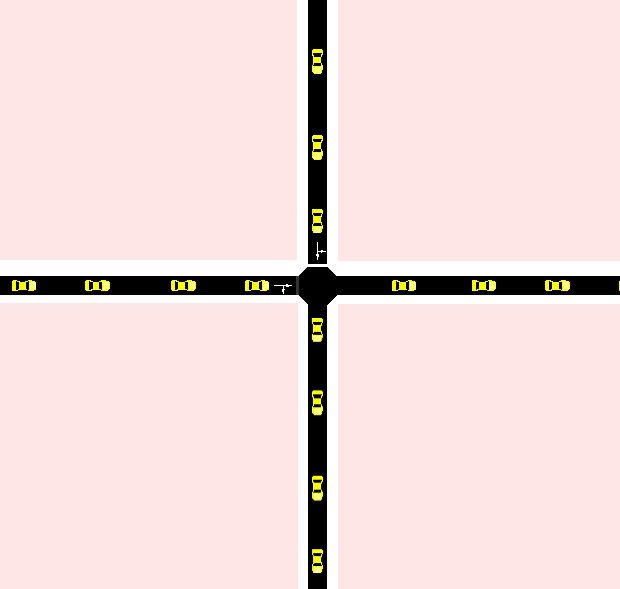
\includegraphics[width=.4\textwidth]{griglia-dettaglio-2.png}
% 	\end{center}
% 	\label{fig:griglia-dettaglio}\caption{Dettaglio della configurazione a griglia: in nero le strade e in giallo gli edifici.}
% \end{figure}
%
\subsection{Risultati}\label{sec:configurazione-griglia-risultati}
%
Come si può vedere dalla Tabella~\ref{tab:risulati-simulazioni-griglia-copertura}
\begin{table}[!h]
	\footnotesize
	\centering
	\begin{tabular}{| L{.2\linewidth} | l | C{.15\linewidth} | C{.15\linewidth} |}
		\toprule
		\multicolumn{2}{|l|}{\multirow{2}{*}{Protocollo e raggio trasmissivo}}	&		\multicolumn{2}{c|}{Copertura totale} 		\\	\cline{3-4}
		\multicolumn{2}{|l|}{}																									&		Senza edifici				& 	Con edifici				\\
		\thickerline
		\multirow{2}{*}{Fast Broadcast}		&	$300$m															&			$97,46$\%					&			$92,66$\%					\\ \cline{2-4}
																			&	$500$m															&			$98,14$\%					& 		$94,27$\%					\\ \hline
		\multirow{2}{*}{\statica}					&	$300$m															&			$92,61$\%					&			$92,66$\%					\\ \cline{2-4}
																			&	$500$m															&			$98,59$\%					& 		$94,25$\%					\\	\hline
		\multirow{2}{*}{\staticb}					&	$300$m															&			$96,54$\%					&			$94,86$\%					\\ \cline{2-4}
																			&	$500$m															&			$98,26$\%					& 		$93,75$\%					\\
		\bottomrule
		\multicolumn{4}{c}{} 	\\
		\toprule
		\multicolumn{2}{|l|}{\multirow{2}{*}{Protocollo e raggio trasmissivo}}	&		\multicolumn{2}{c|}{Copertura sulla circonferenza} 		\\	\cline{3-4}
		\multicolumn{2}{|l|}{}																									&		Senza edifici				& 	Con edifici				\\
		\thickerline
		\multirow{2}{*}{Fast Broadcast}		&	$300$m															&			$97,00$\%					&			$93,00$\%					\\ \cline{2-4}
																			&	$500$m															&			$97,28$\%					& 		$96,78$\%					\\ \hline
		\multirow{2}{*}{\statica}					&	$300$m															&			$97,22$\%					&			$91,65$\%					\\ \cline{2-4}
																			&	$500$m															&			$98,22$\%					& 		$96,33$\%					\\	\hline
		\multirow{2}{*}{\staticb}					&	$300$m															&			$97,17$\%					&			$96,17$\%					\\ \cline{2-4}
																			&	$500$m															&			$97,33$\%					& 		$97,06$\%					\\
		\bottomrule
	\end{tabular}
	\caption{Copertura di veicoli in totale e sulla circonferenza con scenario a griglia.\label{tab:risulati-simulazioni-griglia-copertura}}
\end{table}
%
\section{Scenario urbano reale} % un titolo migliore no?
Le configurazioni precedenti avevano il difetto di essere poco veritiere, sia dal punto di vista della topologia stradale
che sulla geometria degli edifici.
In questo gruppo di simulazioni, invece, si è voluto valutare Fast Broadcast all'interno di uno scenario quanto più reale possibile.
Sono state scelte due città, Padova (IT) e Los Angeles (California, USA) (Figura~\ref{fig:scenari-la-pd-osm}), definite due aree nella zona centrale di circa $5$ kilometri quadrati (Figura~\ref{fig:scenari-la-pd-osm})
e, seguendo il procedimento descritto nella Sezione~\ref{sec:sumo}, si sono estratte le informazioni necessarie alla simulazione.
Altre informazioni sulla configurazione sono elencati in Tabella~\ref{tab:parametri-simulazioni-pd-la}.

La scelta è ricaduta su Los Angeles poiché la sua rete stradale è molto simile a una griglia in stile Manhattan, come anche nello scenario precedente,
mentre Padova (sede anche dell'Università dove si è svolto questo lavoro) ha una toplogià più irregolare, con strade più strette ed edifici a ridosso di queste,
zone pedonali e ZTL.
%
\begin{table}[htbp]
	\centering
	  \begin{tabular}{| L{.35\linewidth} | C{.01\linewidth} | C{.04\linewidth} | L{.15\linewidth} | L{.15\linewidth} |}
			\toprule
			\multicolumn{3}{|m{.3\linewidth}|}{\multirow{2}{*}{}}														&		\multicolumn{2}{c|}{Scenario}						\\ \cline{4-5}
			\multicolumn{3}{|m{.3\linewidth}|}{}																						&		Padova				&			Los Angeles					\\
			\thickerline
			\multicolumn{2}{|m{.25\linewidth}|}{\multirow{2}{*}{Latitudine}}				&		N	 	& 	$45,4171$				&			$33,9654$					\\ \cline{3-5}
			\multicolumn{2}{|m{.25\linewidth}|}{}																		&		S	 	& 	$45,3981$				&			$33,9478$					\\ \hline
			\multicolumn{2}{|l|}{\multirow{2}{*}{Longitudine}}											&		O	 	& 	$11,8654$				&			-$118,3260$				\\ \cline{3-5}
			\multicolumn{2}{|l|}{}																									&		E	 	& 	$11,8923$				&			-$118,3055$				\\ \hline
			\multicolumn{3}{|l|}{Area approssimativa [km$^2$]}															&		\multicolumn{2}{c|}{$5$}								\\ \hline
			\multicolumn{3}{|l|}{Distanza fra veicoli [metri]}															&		\multicolumn{2}{c|}{$25$}								\\ \hline
			\multicolumn{3}{|l|}{Numero di veicoli}																					&		$2224$					&					$1905$				\\ \hline
			\multicolumn{3}{|l|}{Numero di edifici}																					&		$6322$					&					$8241$				\\ \hline
			\multicolumn{3}{|l|}{Circonferenza [metri]}																			&		\multicolumn{2}{c|}{$1000\pm25$}				\\ \hline
			\multicolumn{3}{|l|}{Posizione del veicolo zero}																&		\multicolumn{2}{c|}{centrale}						\\ \hline
			\multicolumn{3}{|l|}{Numero di simulazioni}																			&		\multicolumn{2}{c|}{$50$}								\\
			\bottomrule
	  \end{tabular}
	\caption{Parametri della topologia per gli scenari urbani.\label{tab:parametri-simulazioni-pd-la}}
\end{table}
%
\begin{figure}[htbp]
	\centering
		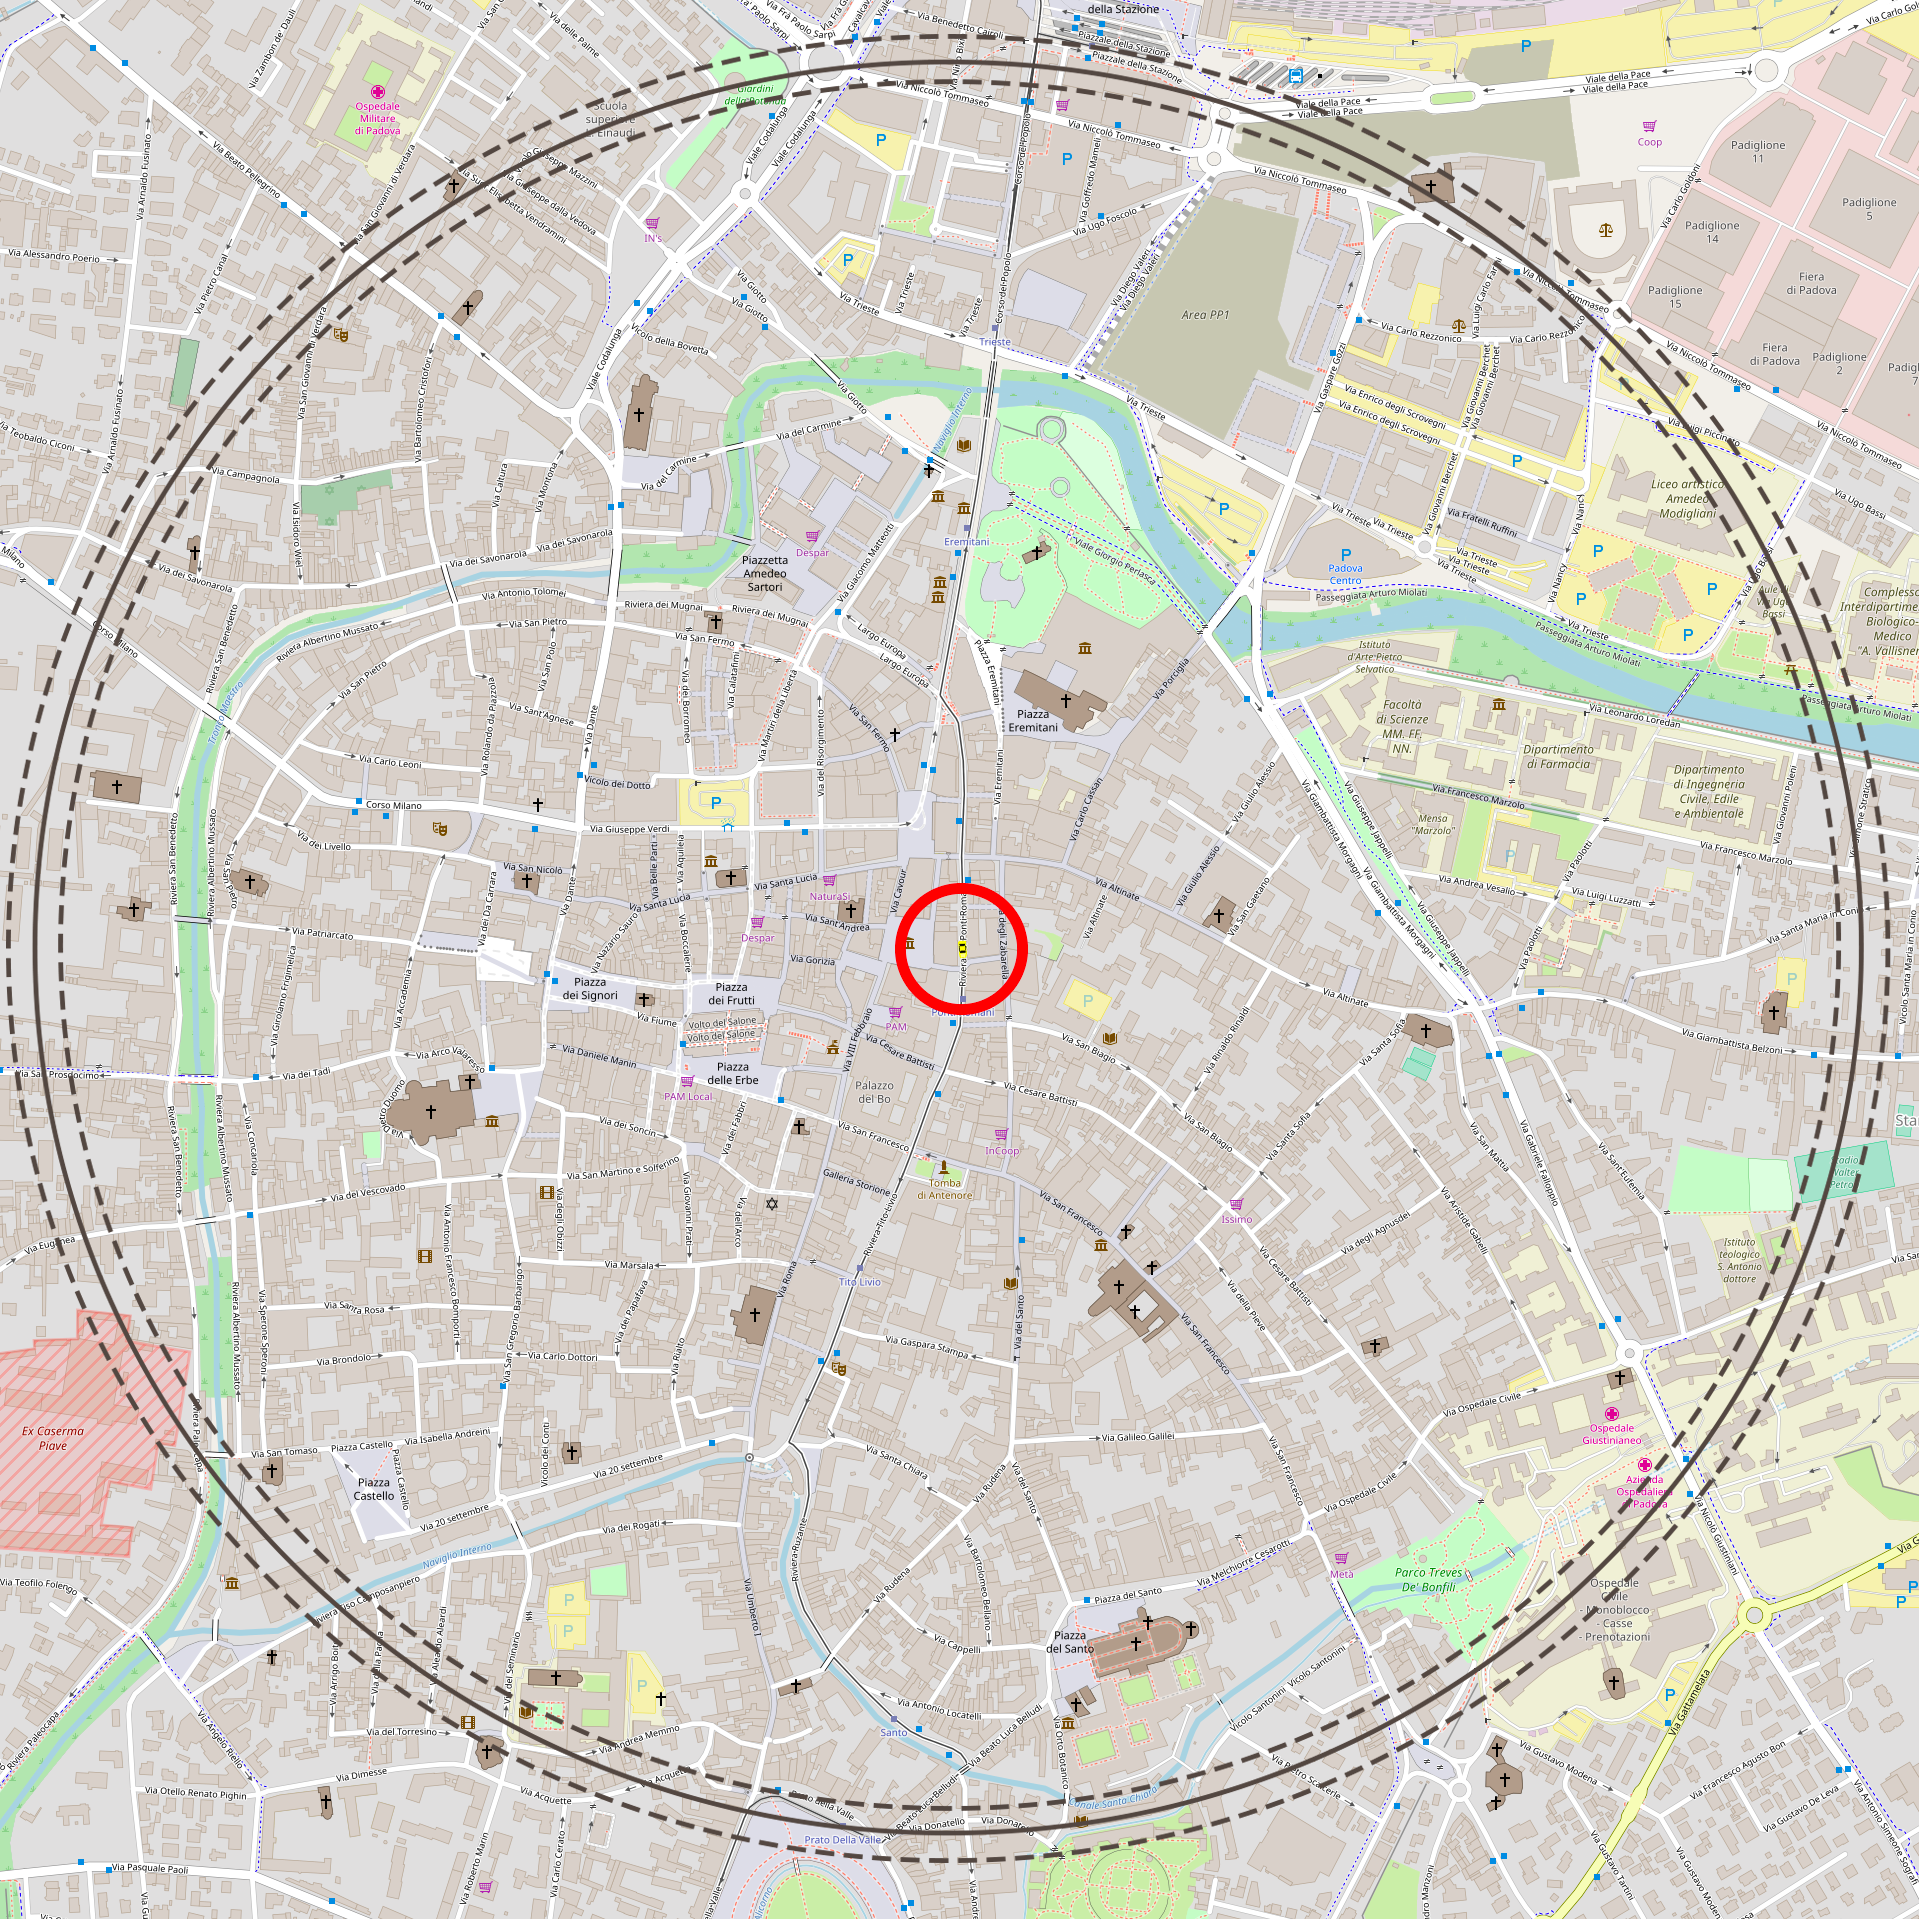
\includegraphics[width=.49\textwidth]{osm_web-pd-2x2.png}
		\hfill
		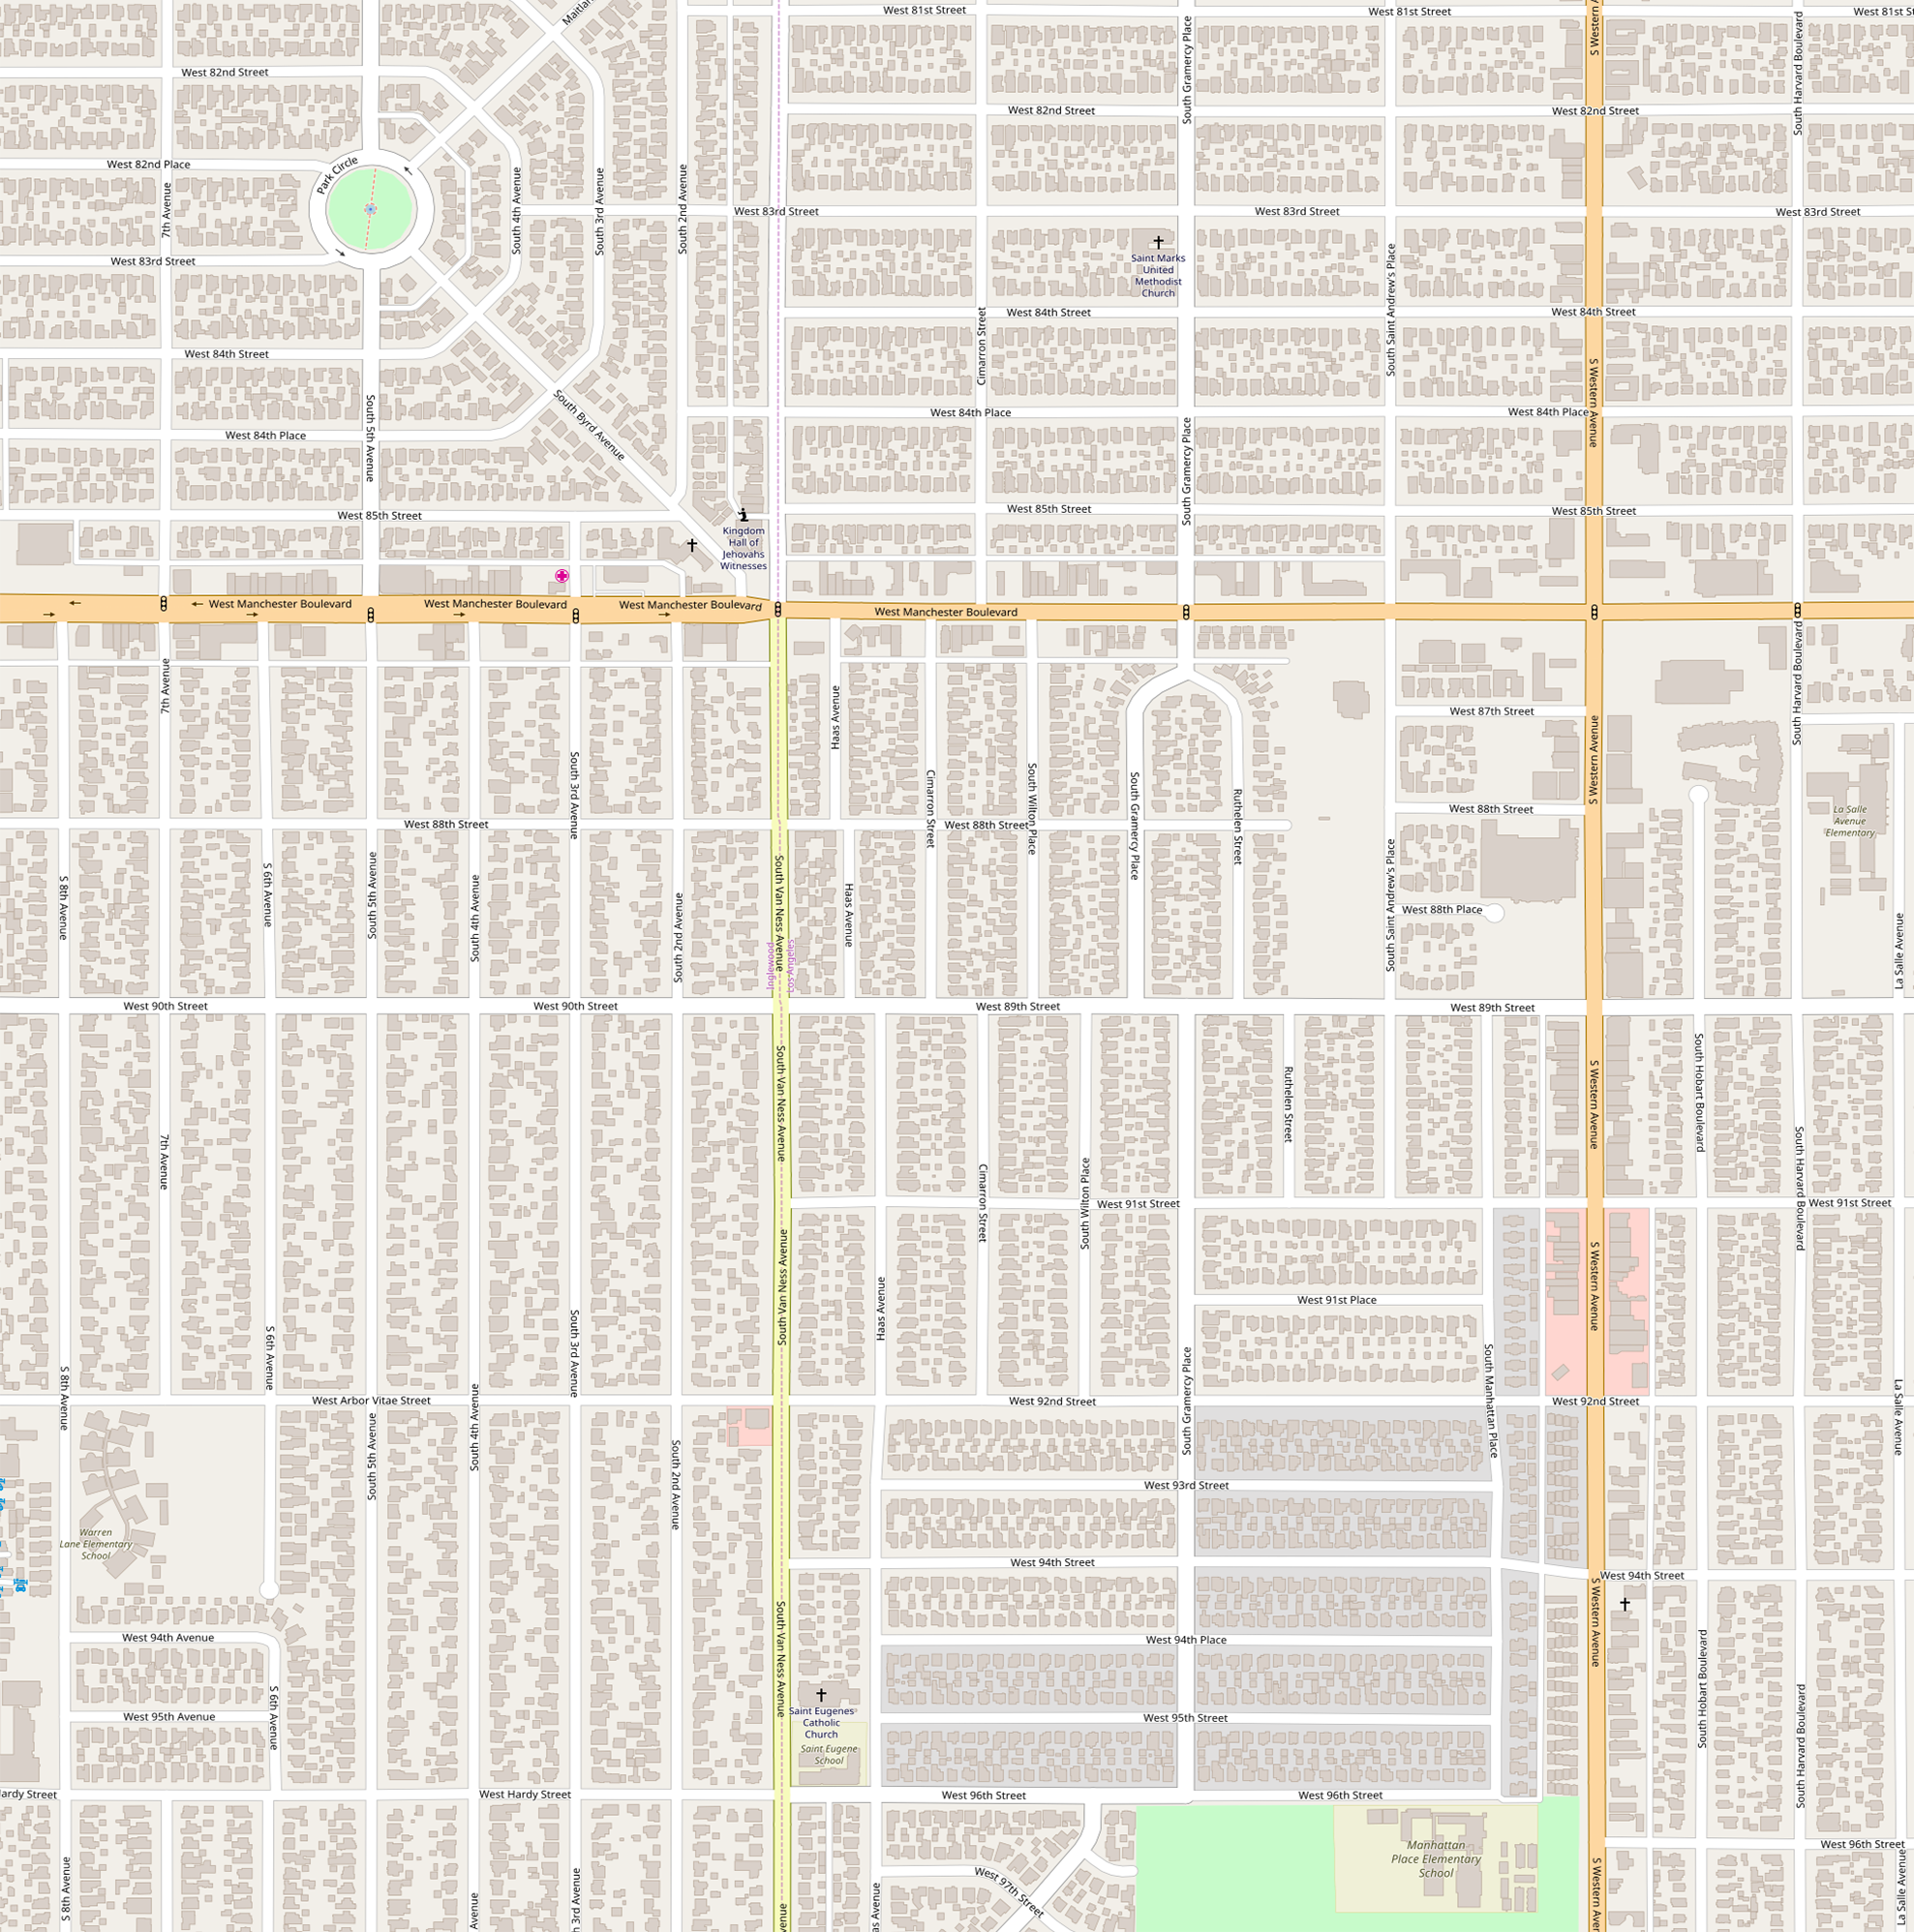
\includegraphics[width=.49\textwidth]{osm_web-la-2x2.png}
\caption{Una vista delle aree selezionate per le simulazioni; a sinistra la città di Padova e a destra Los Angeles (fonte: OSM).
Il cerchio rosso evidenzia la posizione del nodo di partenza mentre i tre rimanenti rappresentano il perimetro della circonferenza
e i due intervalli di confidenza.\label{fig:scenari-la-pd-osm}}
\end{figure}
%
Anche in questo gruppo di simulazioni sono state utilizzate le medesime metriche del caso precendente,
fatta eccezione per il numero di salti che ora sono per raggiungere la circonferenza, non il bordo dello scenario.
Questo perché nella configurazione a griglia lungo il perimetro esterno erano sicuramente posizionati dei veicoli,
mentre ora il limite ``quadratico'' dell'area è ideale (non tutte le strade finisco esattamente sul bordo della mappa).
%
\subsection{Los Angeles}\label{subsec:risultati-la}
%
\subsection{Padova}\label{subsec:risultati-pd}

% \begin{figure}[htbp]
% 	\centering
% 		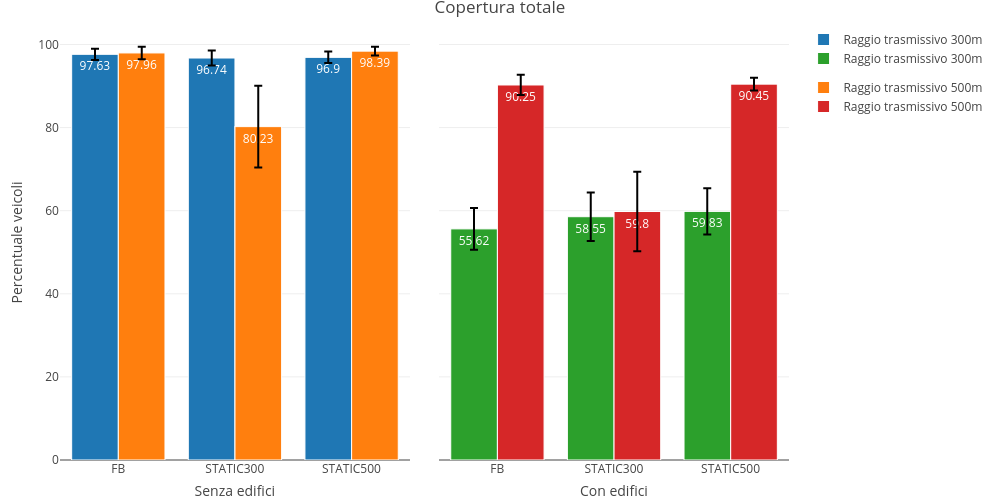
\includegraphics[width=\textwidth]{grafici/pd_copertura_totale.png}
% 		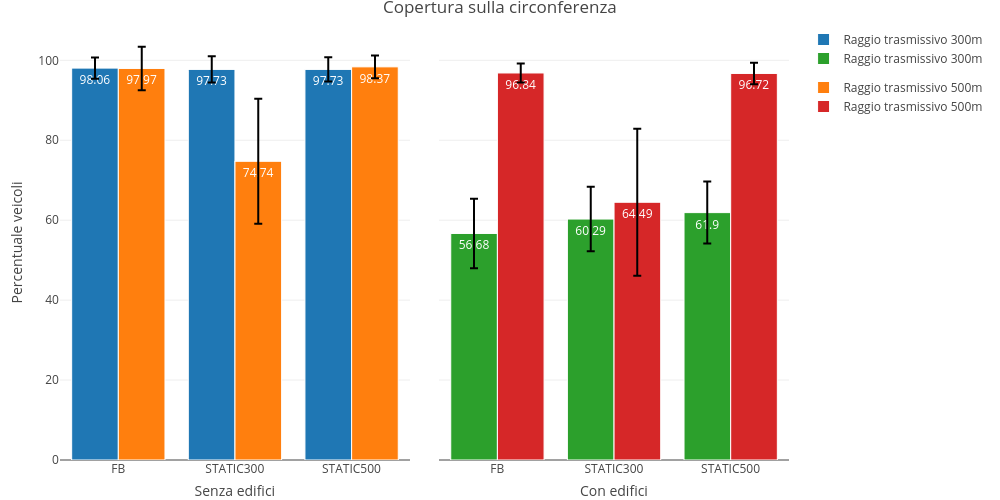
\includegraphics[width=\textwidth]{grafici/pd_copertura_circonferenza.png}
% \caption{Copertura dei veicoli totale e sulla circonferenza dei veicoli\label{fig:risultati-padova-copertura}}
% \end{figure}
% %
% \begin{figure}[htbp]
% 	\centering
% 		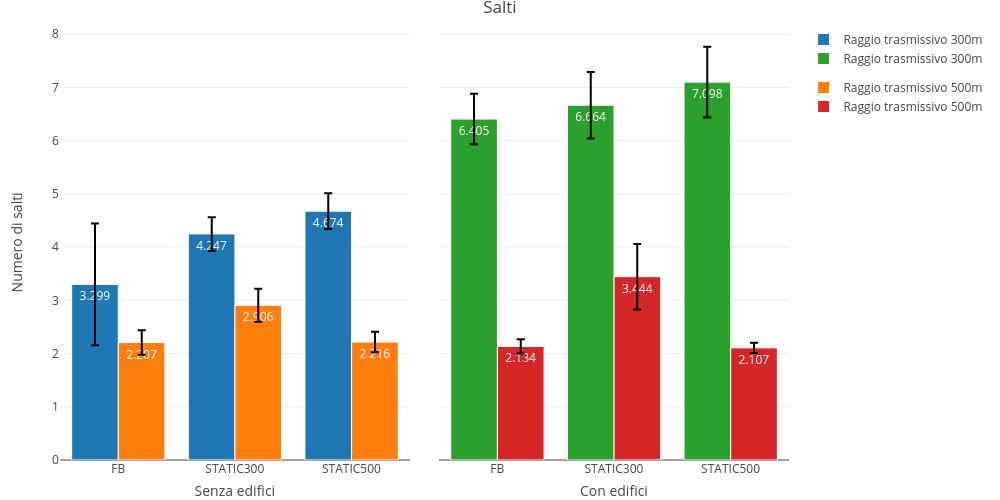
\includegraphics[width=\textwidth]{grafici/pd_salti.png}
% \caption{Numero di salti necessario per raggiungere la circonferenza dei veicoli\label{fig:risultati-padova-salti}}
% \end{figure}
% %
% \begin{figure}[htbp]
% 	\centering
% 		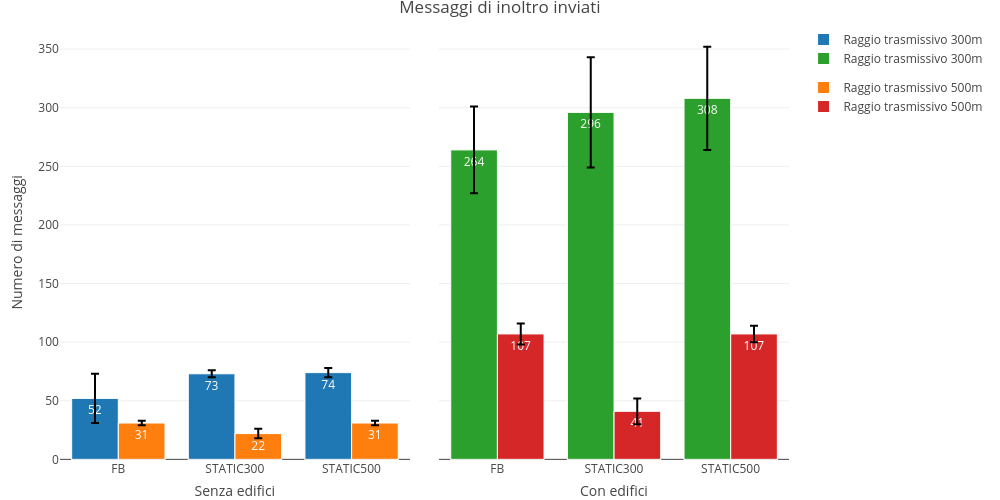
\includegraphics[width=\textwidth]{grafici/pd_messaggi_inviati.png}
% 		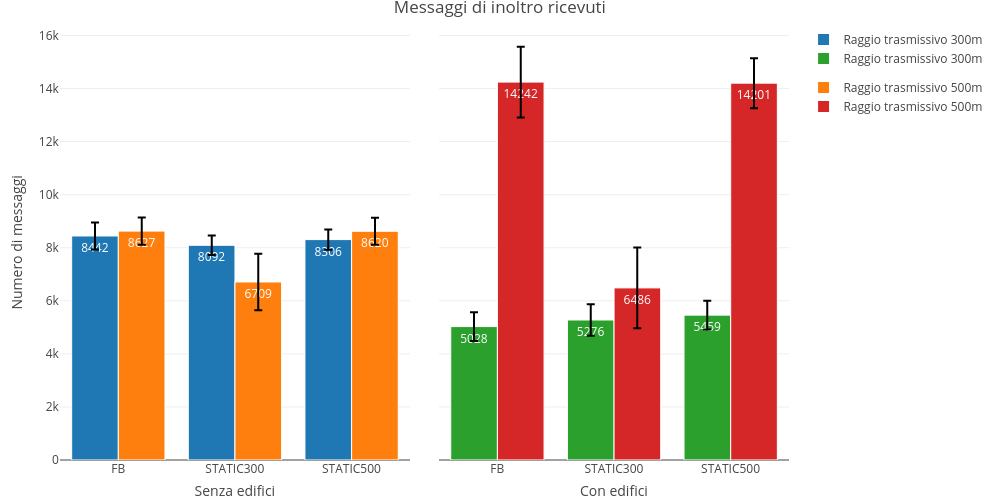
\includegraphics[width=\textwidth]{grafici/pd_messaggi_ricevuti.png}
% \caption{Quantità di messaggi di inoltro durante la simulazione.\label{fig:risultati-padova-messaggi}}
% \end{figure}
